\section{Structural Pipeline}

The construction of the Thalean graph reveals a clear structural pipeline.
Starting from the $60$-vertex chamber graph $G_{60}$, a Klein four symmetry
acts on the vertex set, producing $15$ orbits of size four. Collapsing these
orbits yields a quotient graph $Q_{15}$ which is isomorphic to the line graph
of the Petersen graph.

\begin{figure}[h]
\centering

\begin{tabular}{cc}

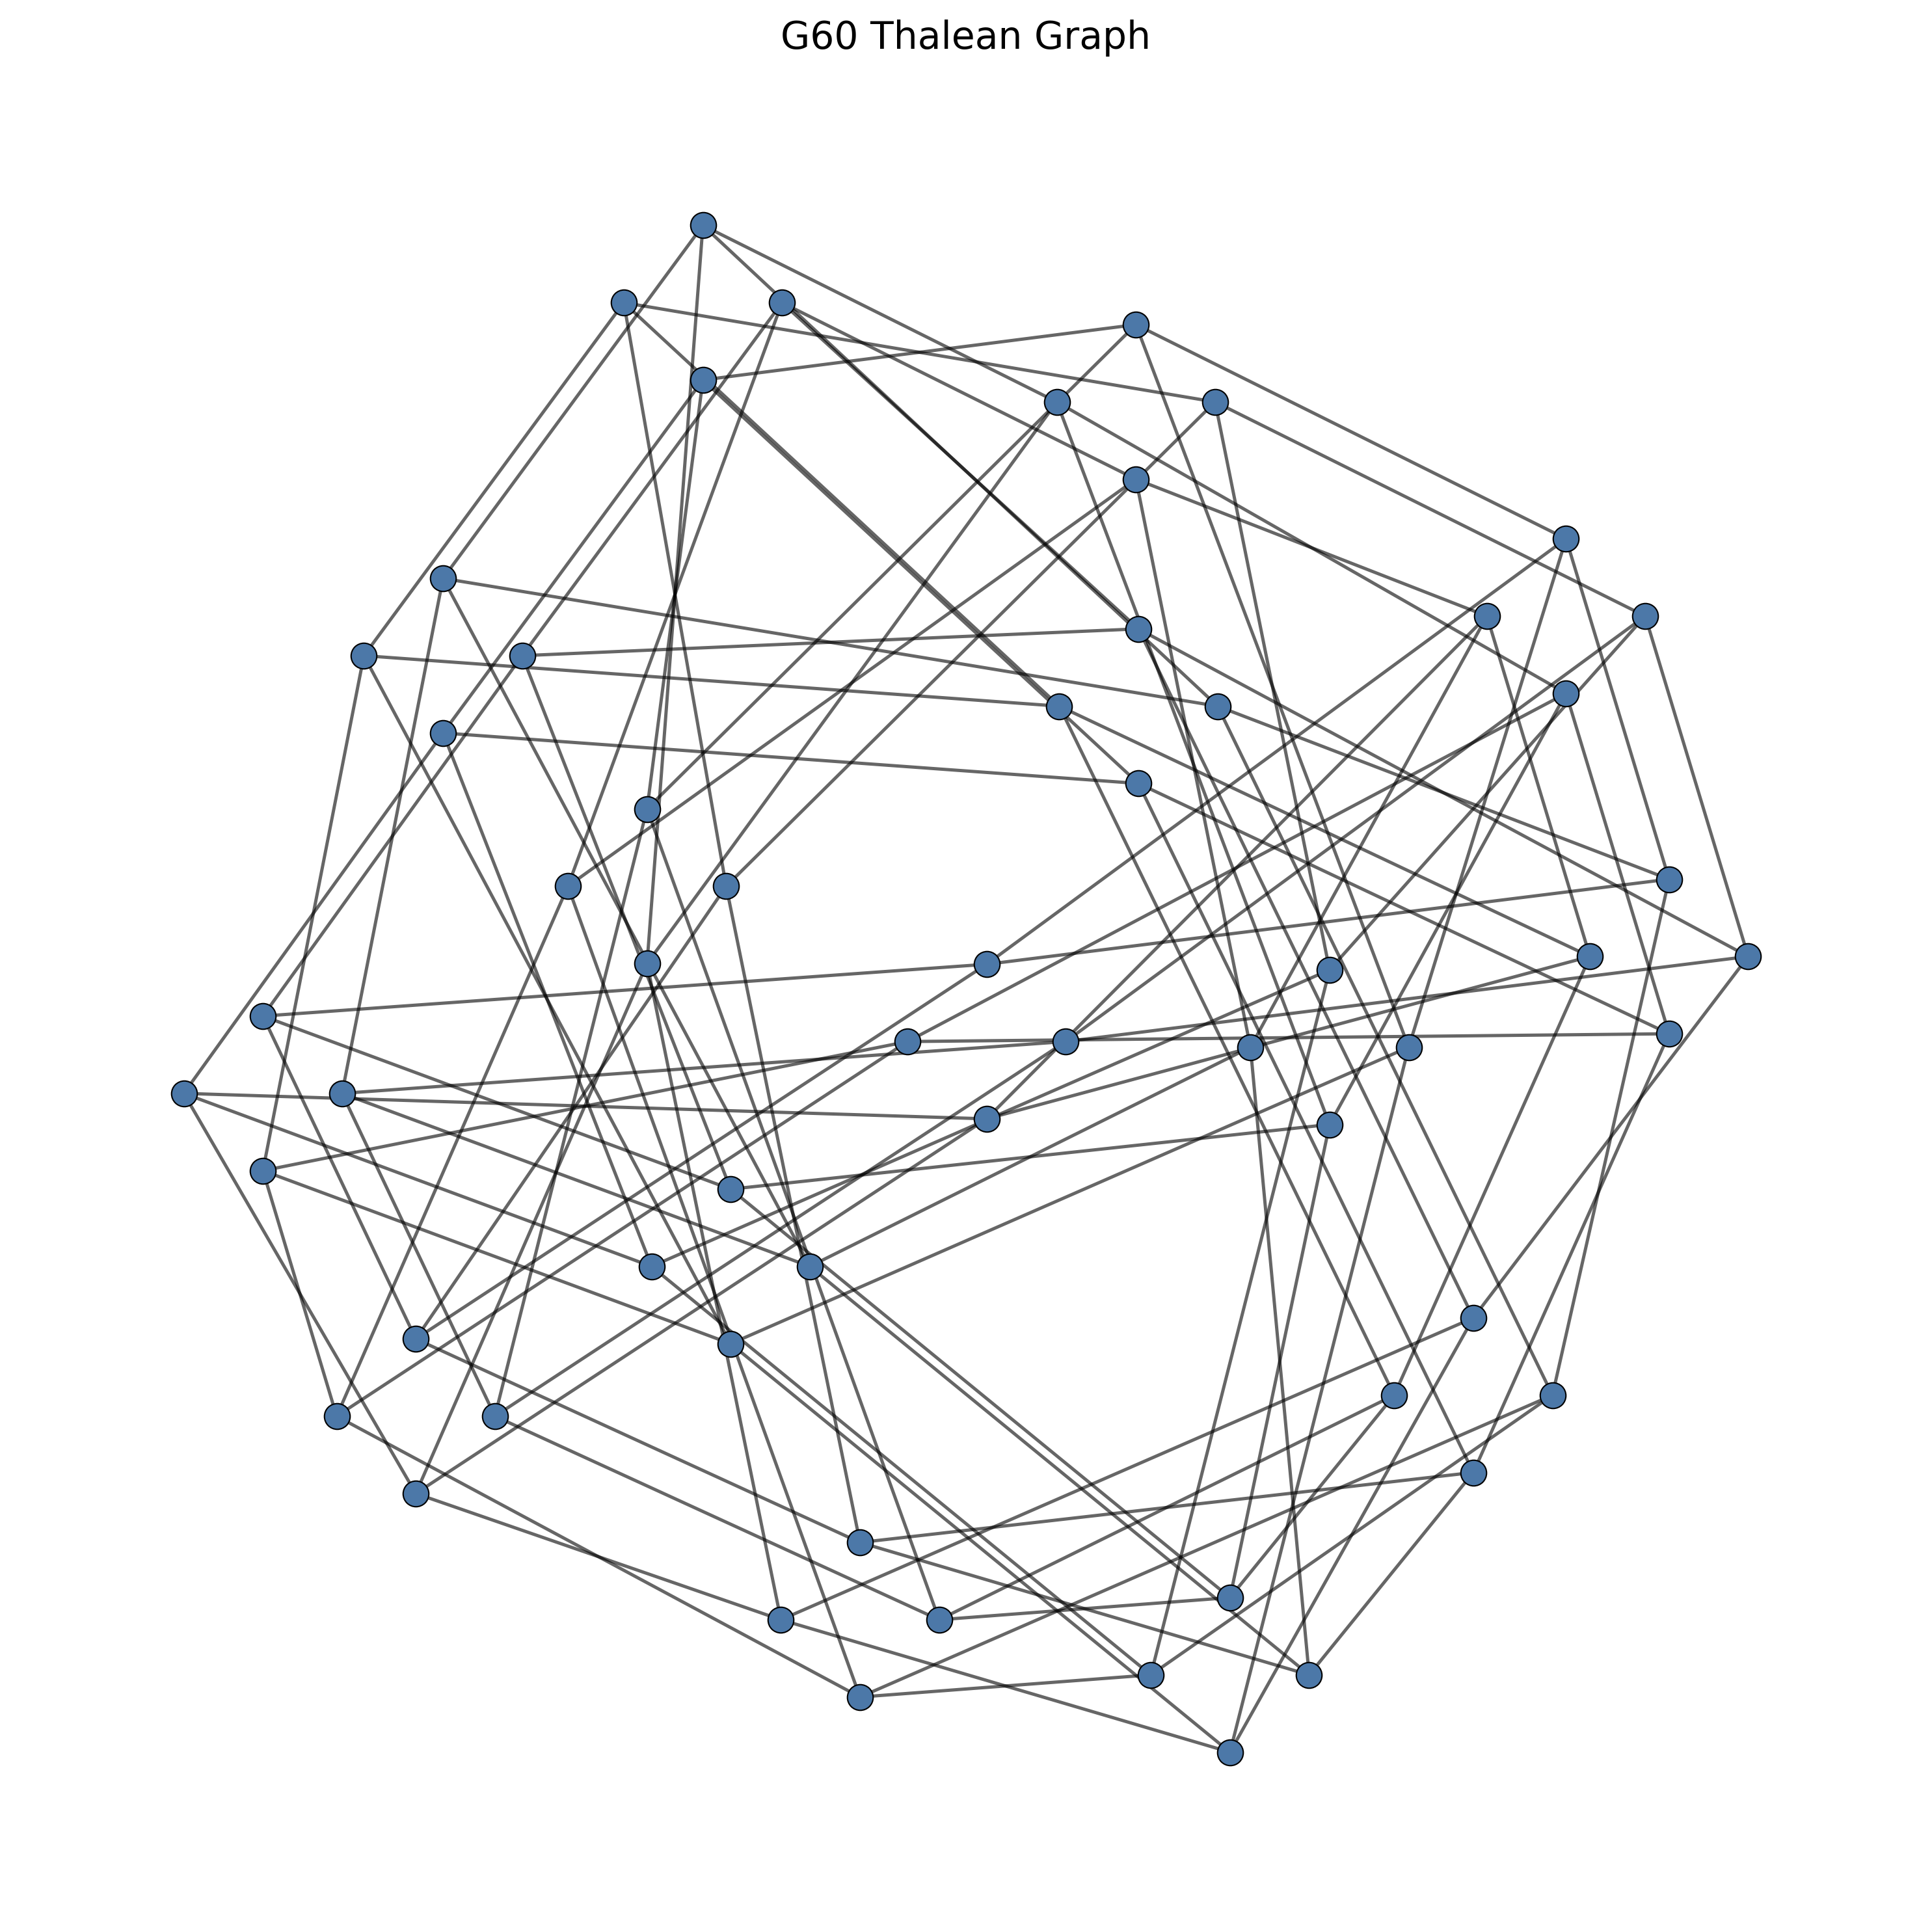
\includegraphics[width=0.42\linewidth]{figures/g60_graph.png} &
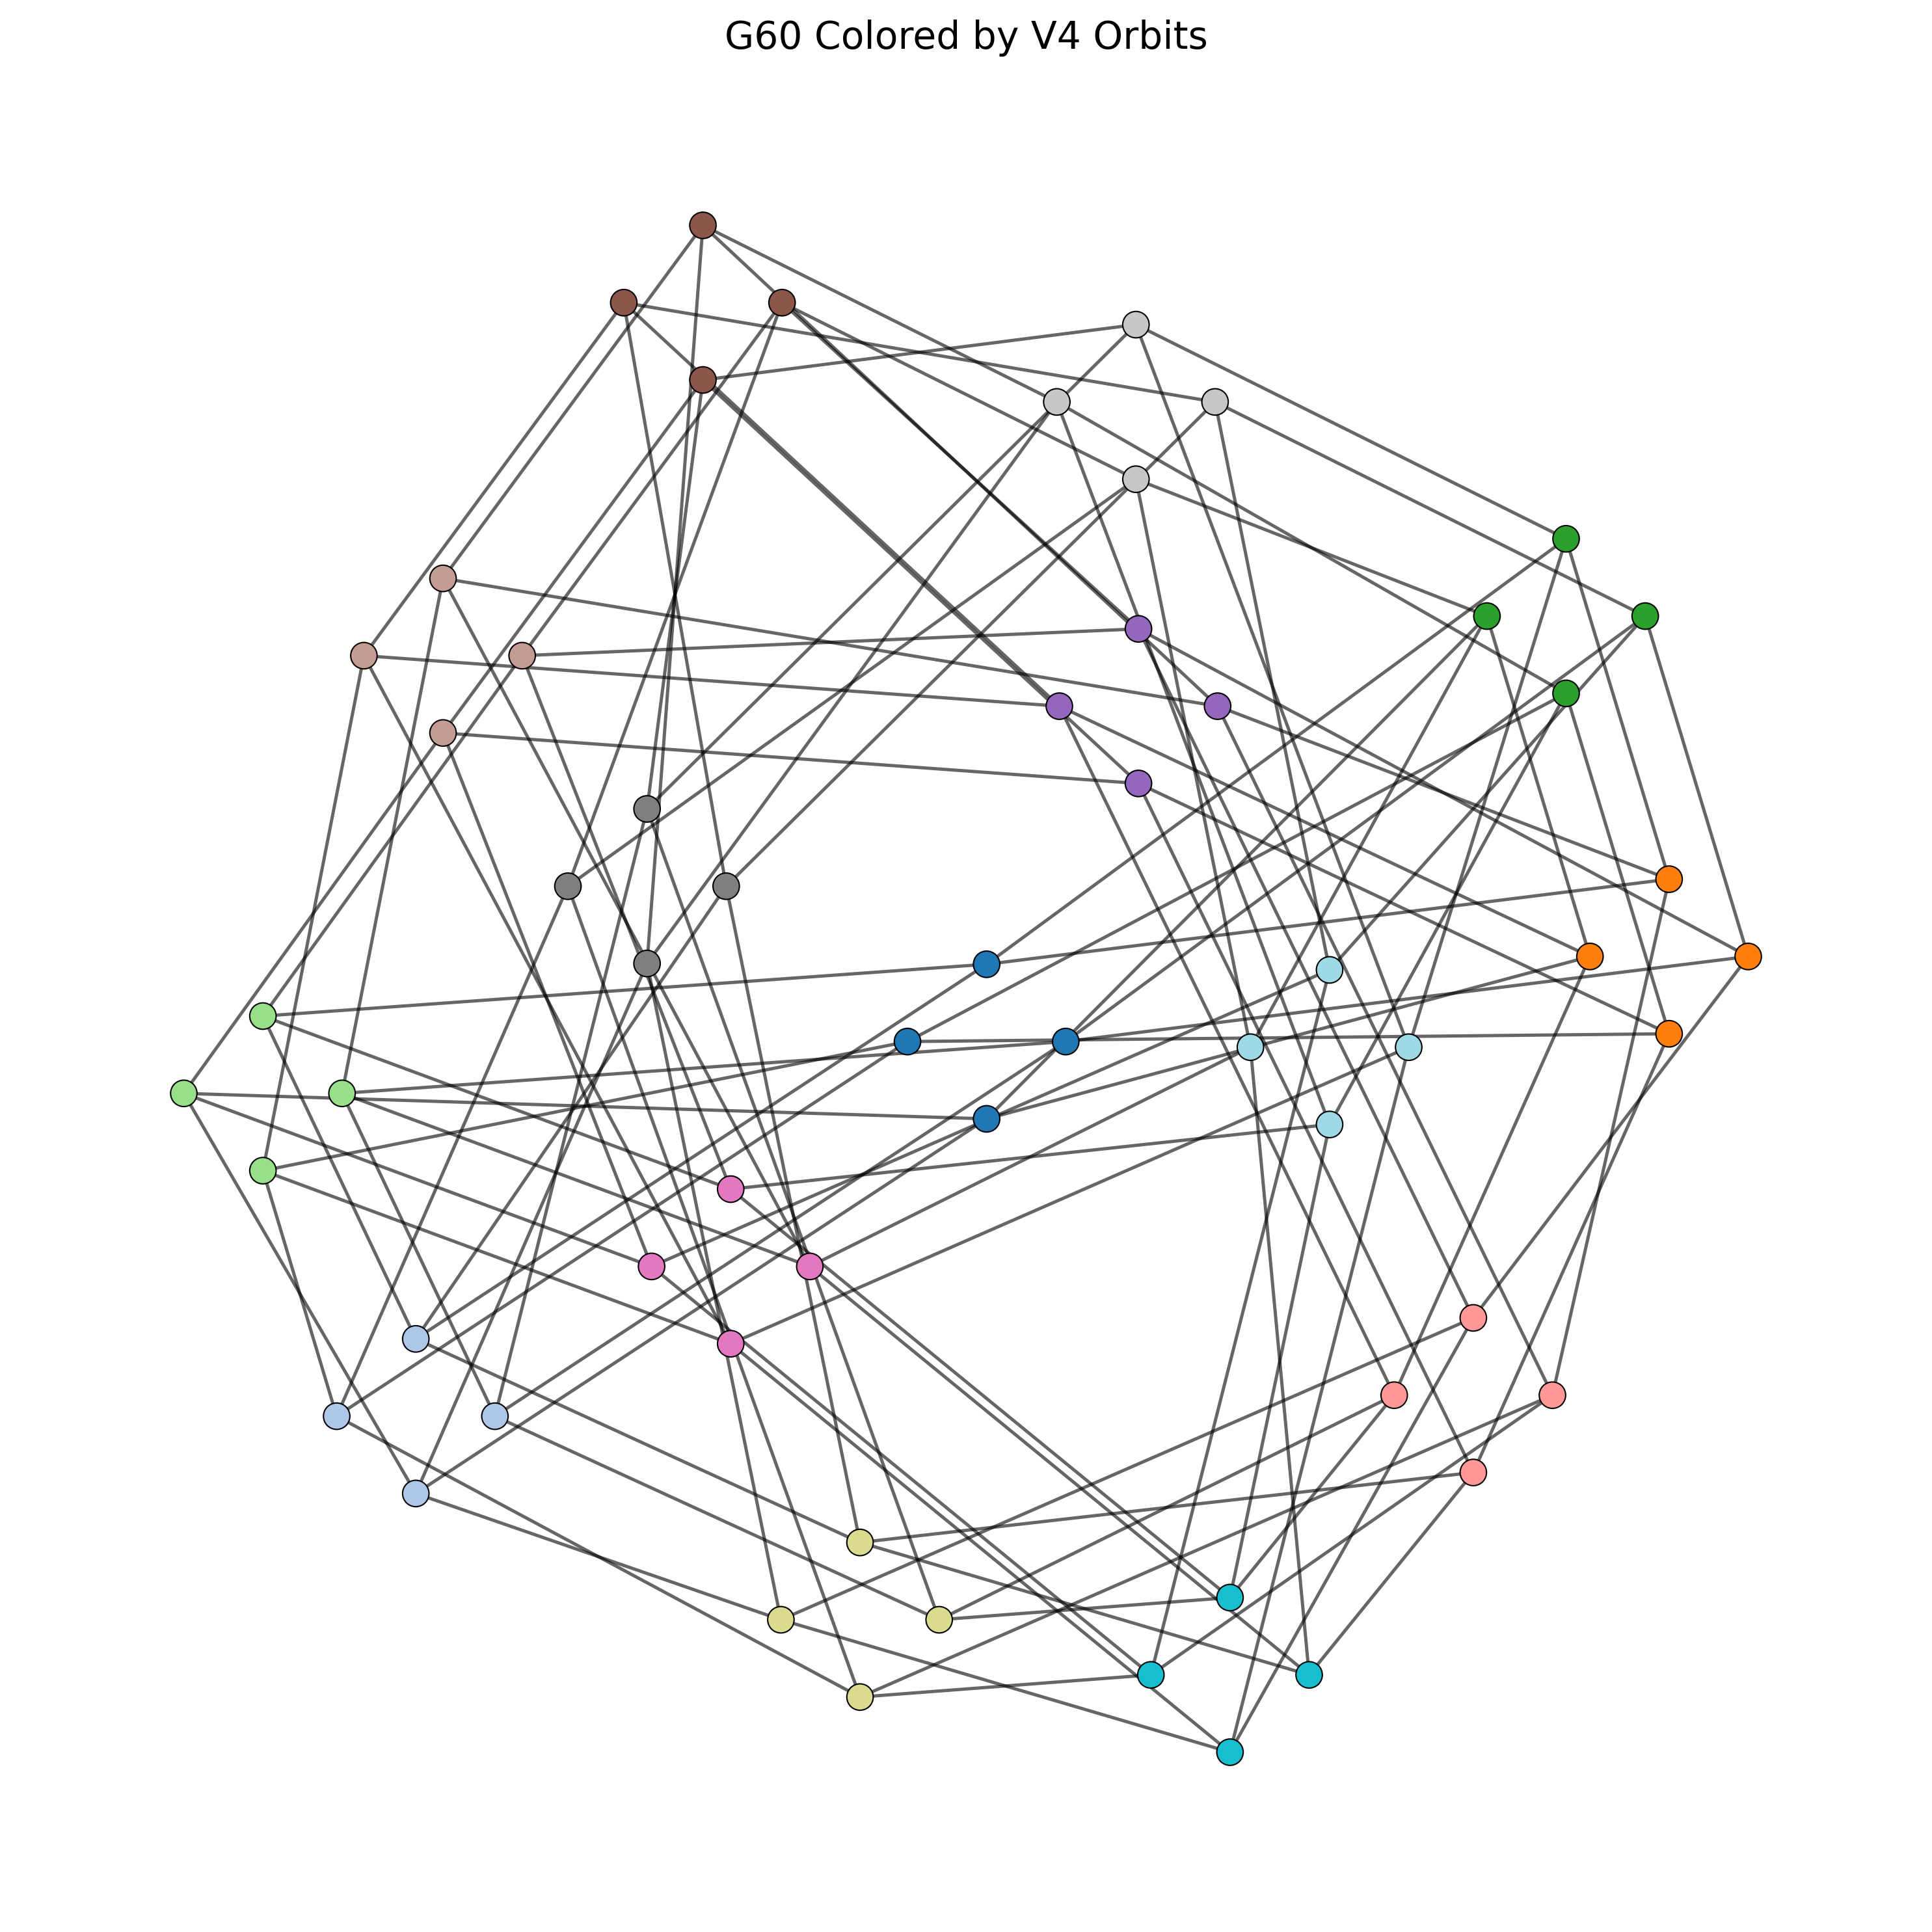
\includegraphics[width=0.42\linewidth]{figures/g60_v4_orbits.png} \\

(a) $G_{60}$ chamber graph &
(b) $V_4$ orbit structure \\

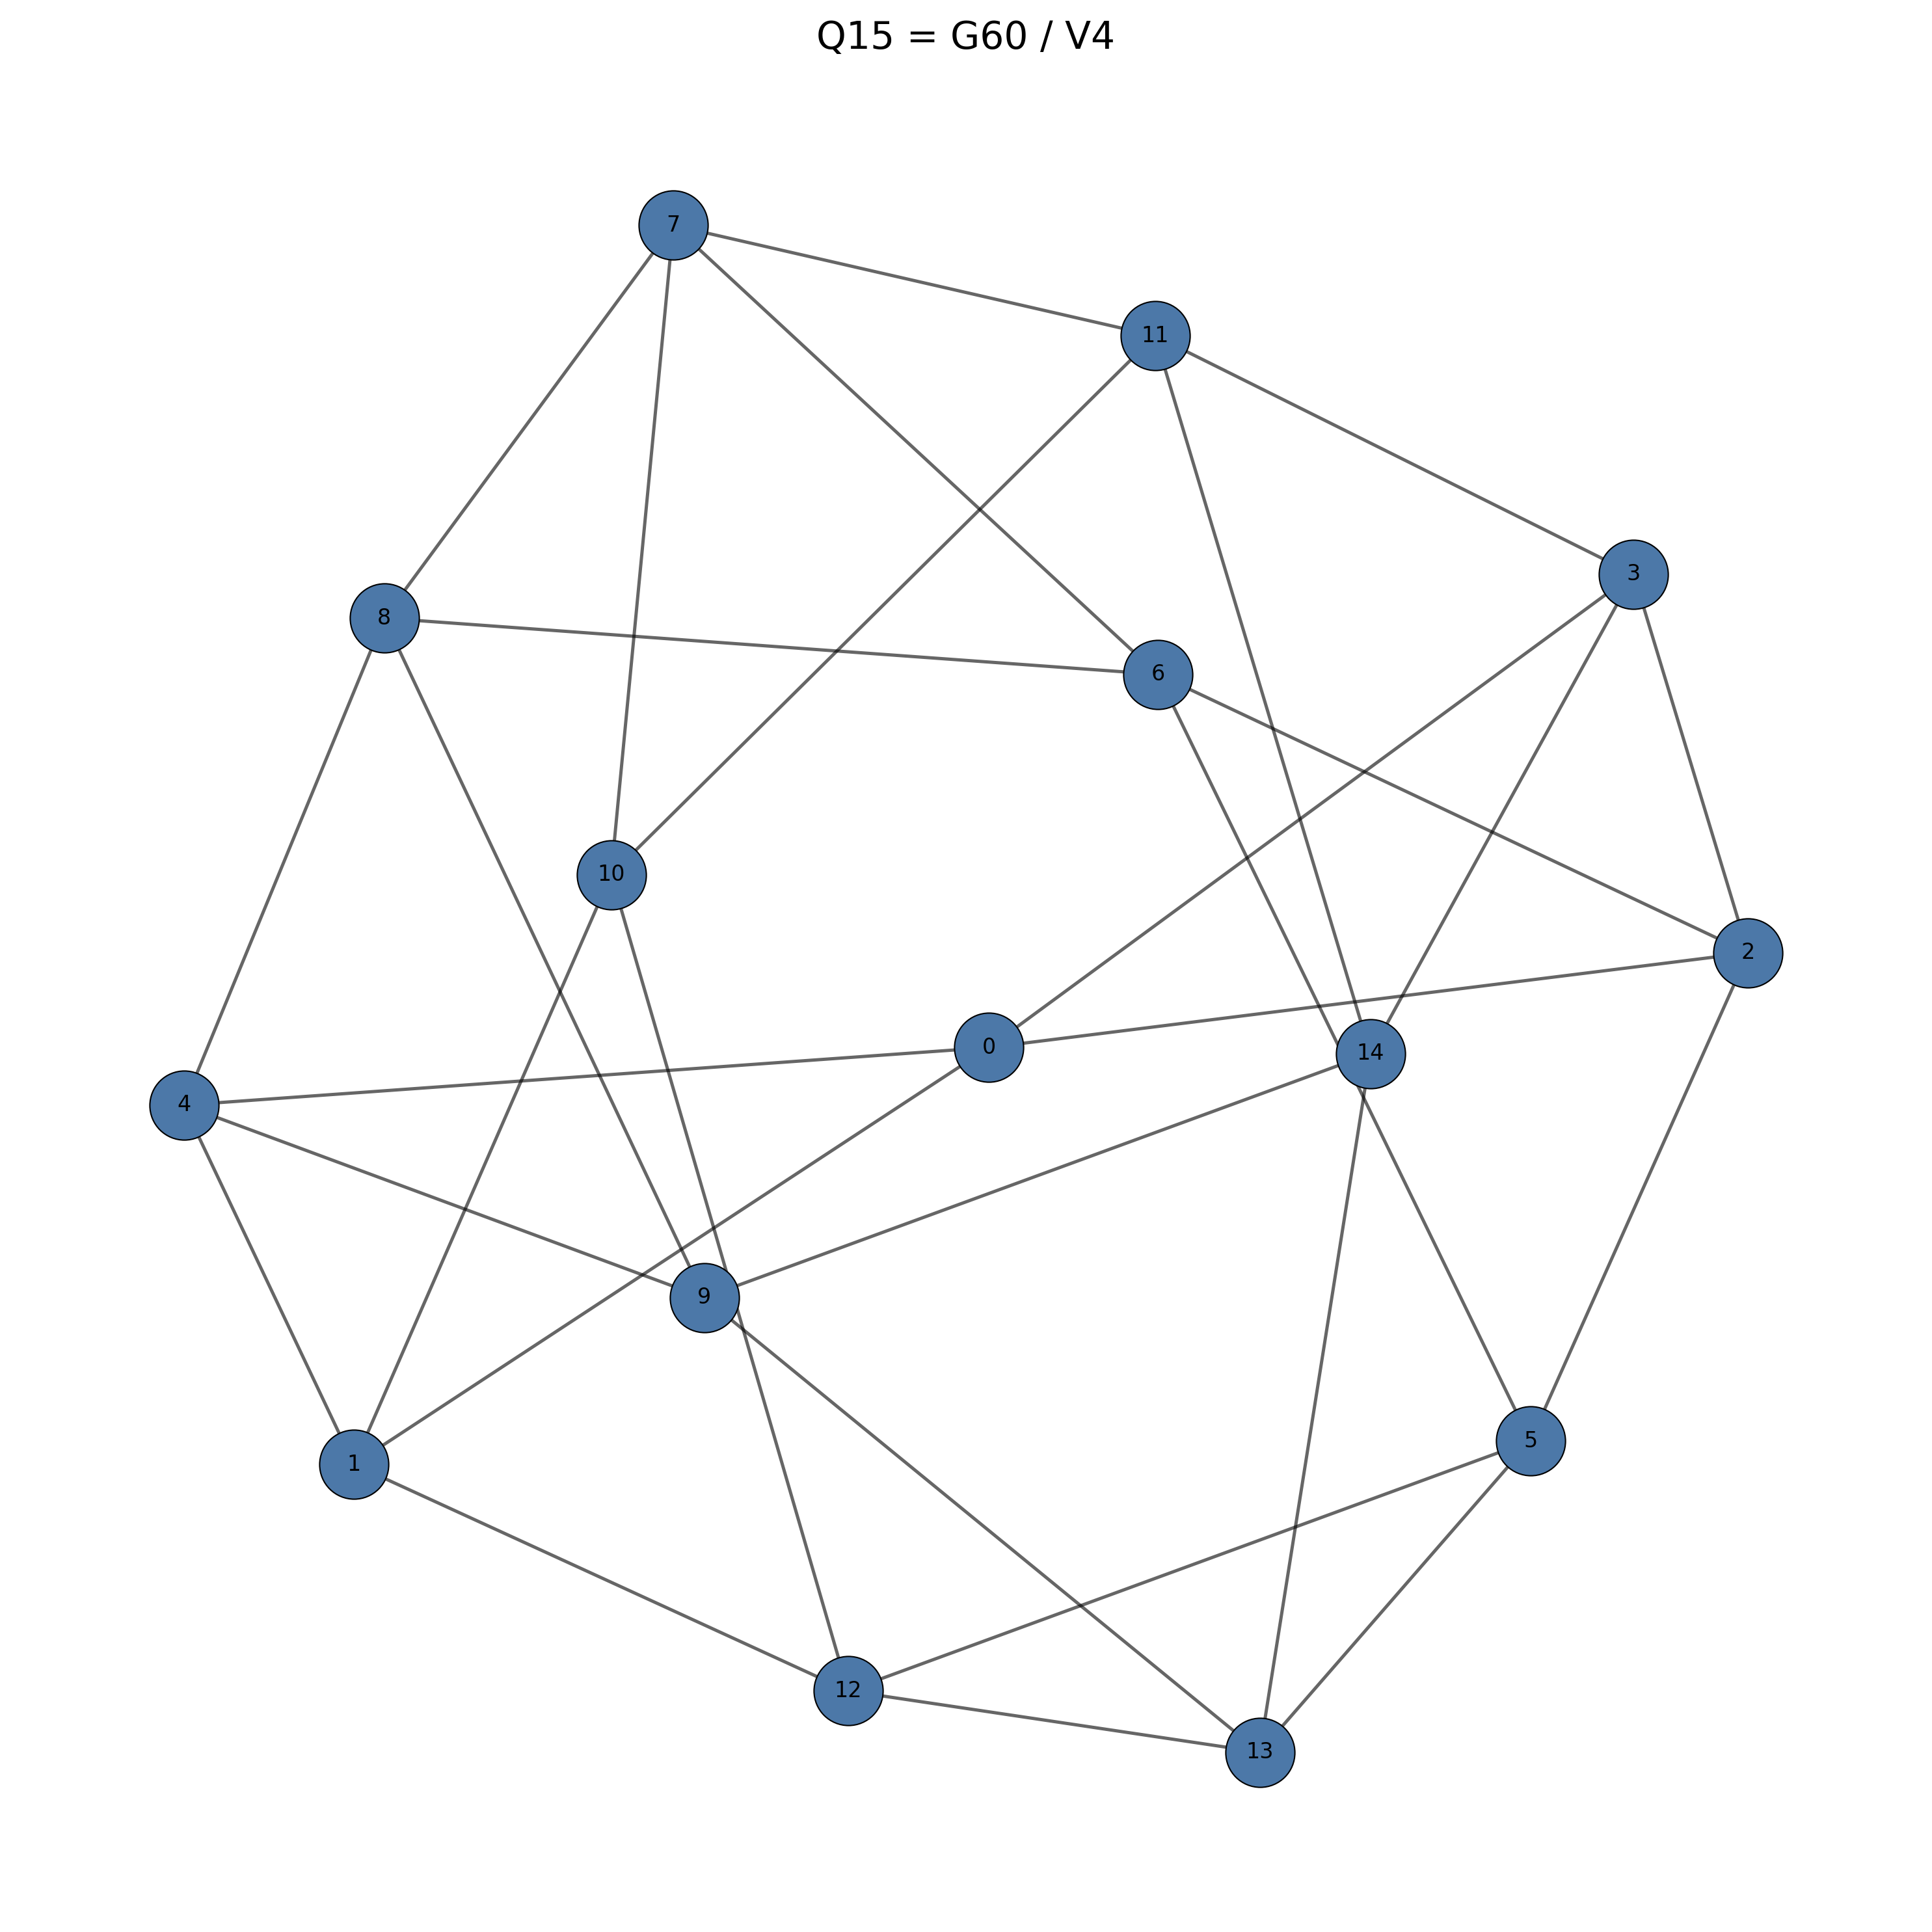
\includegraphics[width=0.42\linewidth]{figures/q15_graph.png} &
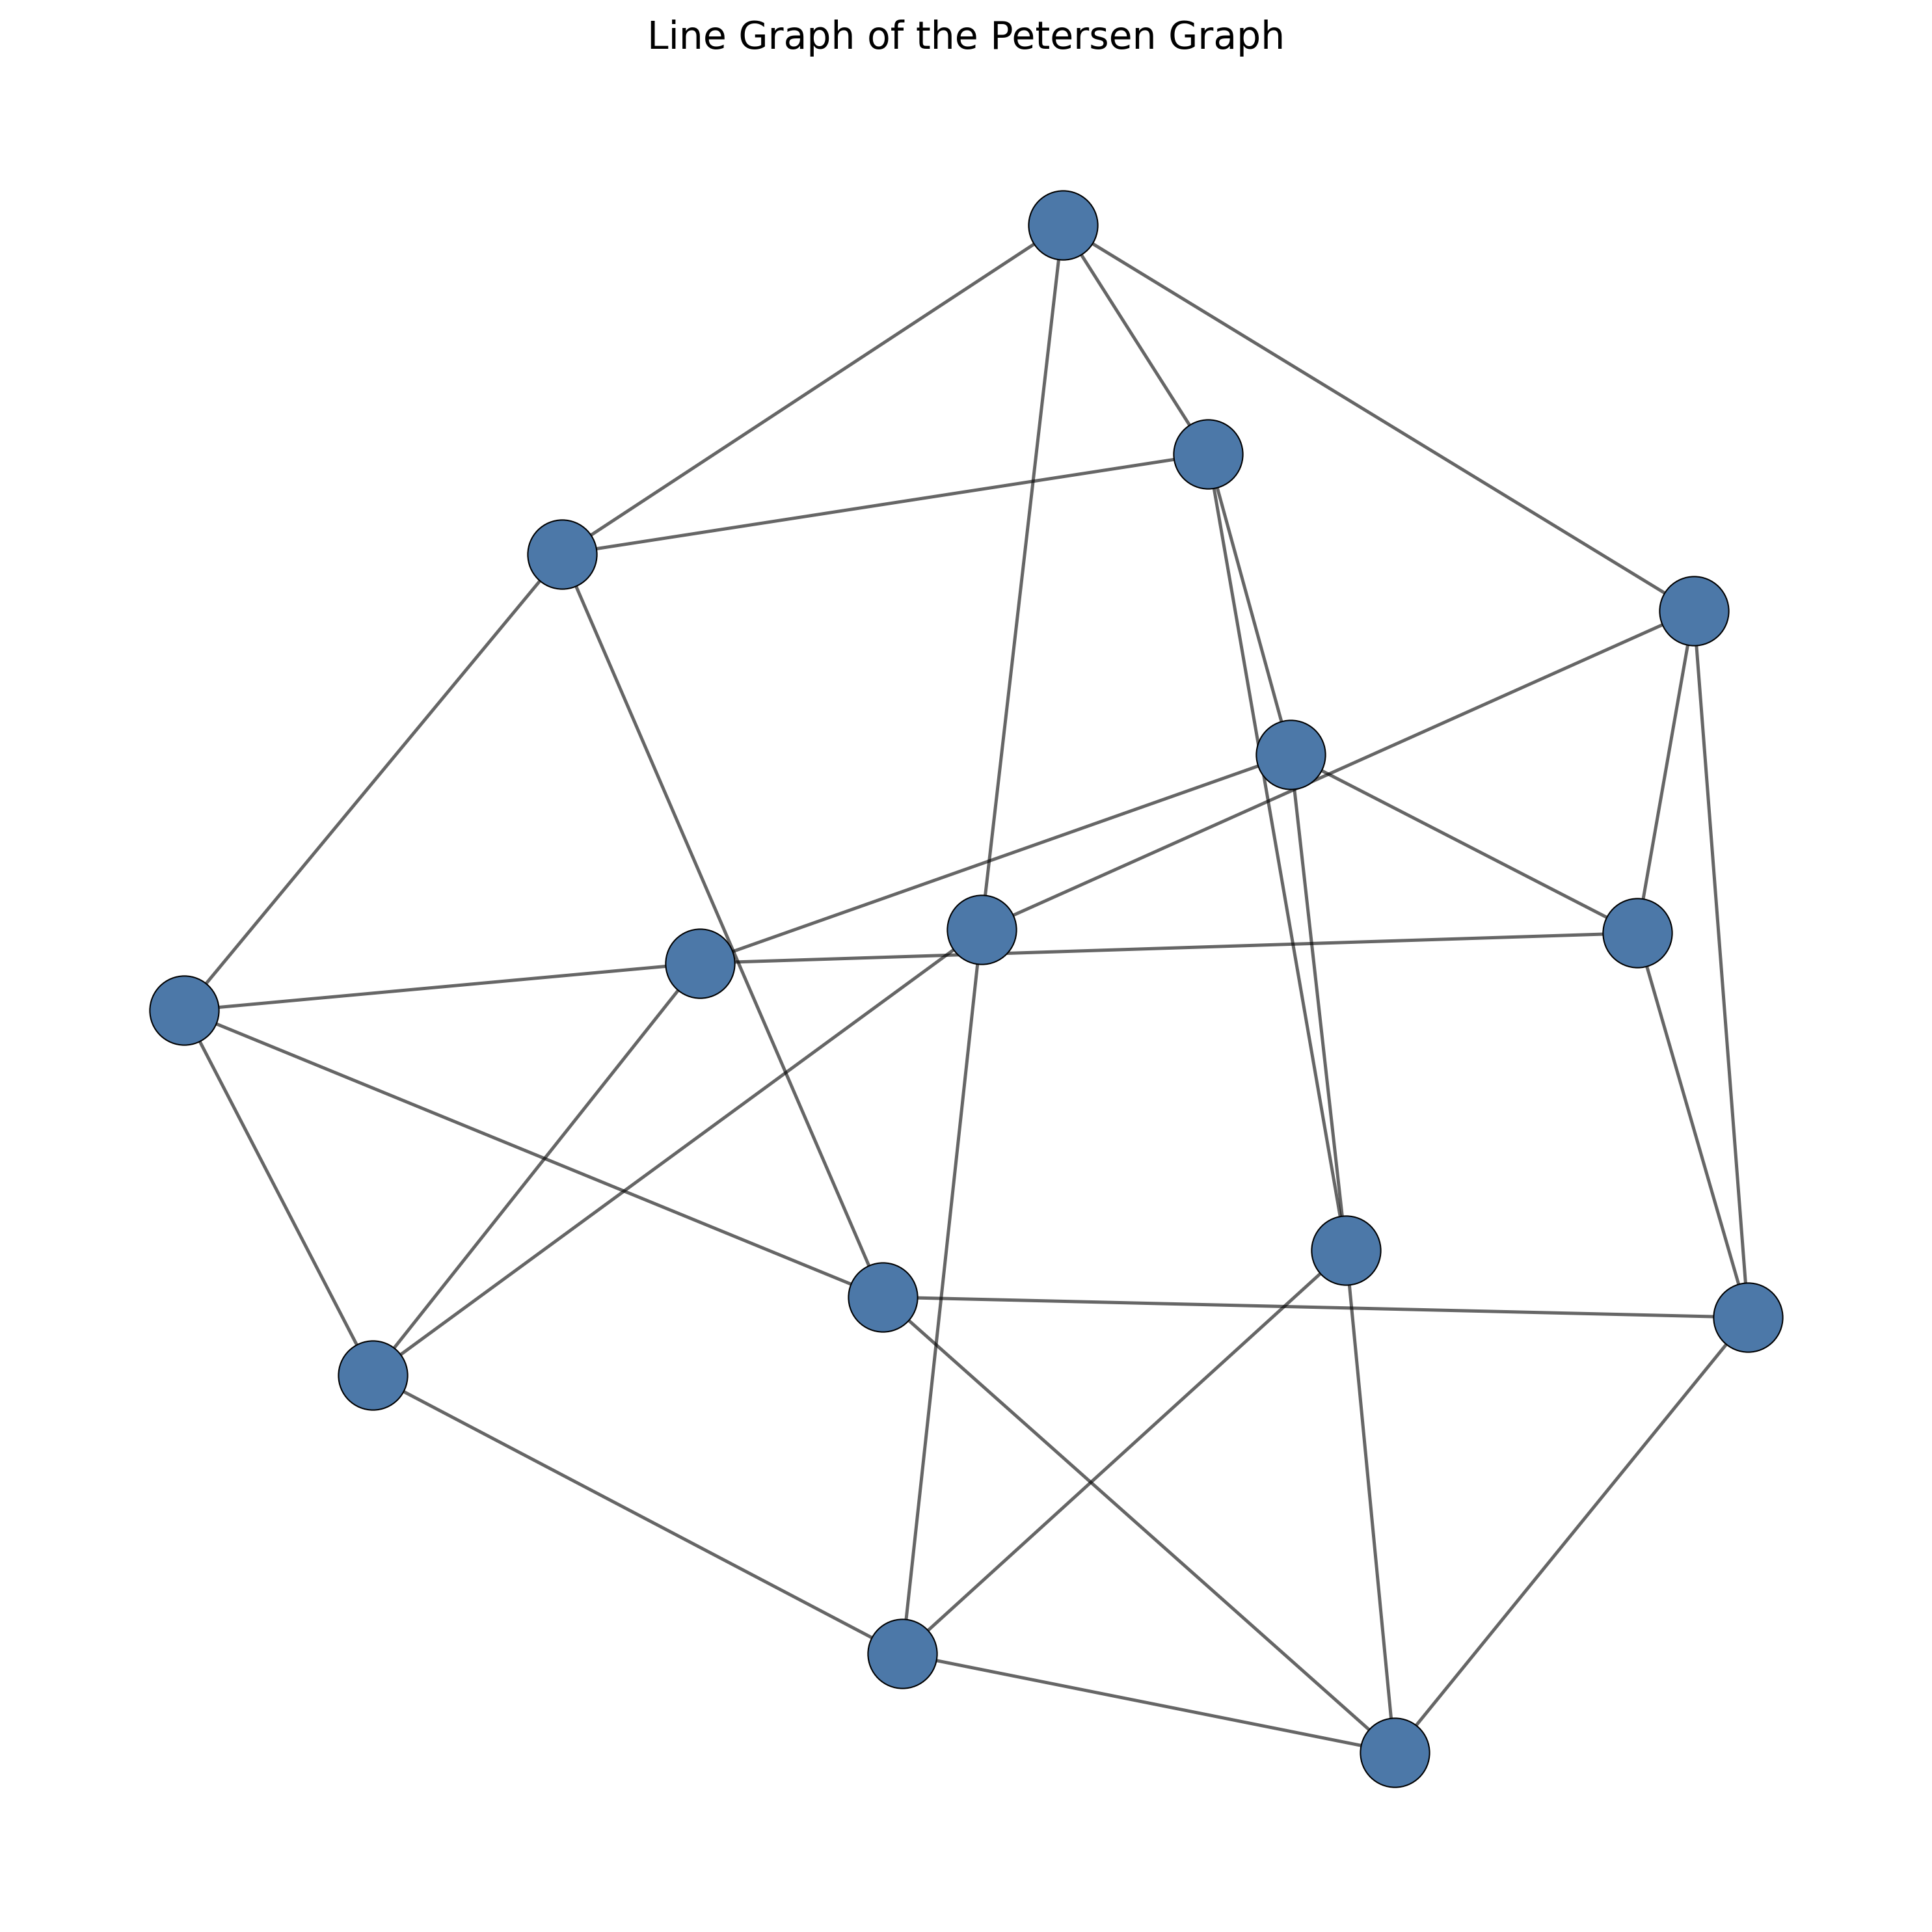
\includegraphics[width=0.42\linewidth]{figures/petersen_line_graph.png} \\

(c) Quotient graph $Q_{15}$ &
(d) $L(\mathrm{Petersen})$

\end{tabular}

\caption{
Structural pipeline of the construction. The Thalean graph $G_{60}$ admits a
$V_4$ symmetry whose orbits collapse to the $15$-vertex graph $Q_{15}$.
Computational verification shows $Q_{15} \cong L(\mathrm{Petersen})$.
}

\label{fig:construction_pipeline}

\end{figure}

